\documentclass[11pt]{article}
\usepackage[margin=1in]{geometry}
\usepackage{graphicx,longtable,array,amsmath,url}
\setlength{\parskip}{4pt}
\title{\textbf{Mammalian-jump mutations in the PB1 and PA polymerase subunits of H5N1 clade 2.3.4.4b: a locked-gate enrichment analysis of 71,778 isolates with structural mapping onto the polymerase--ANP32B complex}}
\author{Computational analysis pipeline (builder 2, PB1/PA slice)\\
H5N1 mammal-jump project, open-data biocomputation program}
\date{September 23, 2026}
\begin{document}
\maketitle
\begin{abstract}
\textbf{Background.} Highly pathogenic avian influenza A(H5N1) clade 2.3.4.4b has caused an unprecedented panzootic with repeated spillover into mammals, including the 2024--2026 United States dairy-cattle outbreak (genotype B3.13), marine-mammal die-offs in South America, and sporadic human cases. The viral polymerase (PB2, PB1, PA) is the principal determinant of avian-to-mammal host adaptation, but most adaptation markers were defined in pre-2.3.4.4b backgrounds.
\textbf{Methods.} We downloaded all H5N1 segment 1--3 records from NCBI GenBank published 2021--2026 (71,778 records; byte-locked with SHA-256 manifests before analysis), classified hosts as natural mammalian ($n\approx5,000$/segment) or avian ($n\approx17,500$/segment), and tested every amino-acid position in PB1 (757 aa) and PA (716 aa) for mammalian enrichment using Fisher exact tests with Benjamini--Hochberg correction, pre-registered effect-size gates (odds ratio $\geq5$, mammalian frequency $\geq5\%$ and $\geq3\times$ avian), and leave-one-host-group-out jackknife. Gates, positive controls (PB2 E627K technical control; PA T97I, PB1 N105S, PB1-F2 N66S as literature-validated controls), and analysis code were frozen before outcomes were examined. Candidate residues were mapped onto the cryo-EM structure of the H5N1 polymerase--human ANP32B complex (PDB 8R1J/8R1L).
\textbf{Results.} The pipeline recovered PB2 E627K (odds ratio 5.9, $q=1.6\times10^{-62}$) and PB1 N105S. Two literature controls failed for biological, not technical, reasons: PA T97I is essentially absent from 2.3.4.4b ($\leq0.11\%$ in both hosts), and PB1-F2 N66S is \emph{reversed}---S66 is fixed in the avian lineage (88.9\%) and depleted in mammals (10.0\%). Five of eleven literature ``mammalian'' markers (PB1 V3, P13, G622, V473; PA D383) are already fixed ($\geq99.7\%$) in the 2.3.4.4b \emph{avian} background: the panzootic lineage is pre-adapted at historical marker positions. High-frequency mammalian enrichments in PB1 (E75D, M171V, M179I, A587P) and PA (K113R, L219I, S277P, K497R, S558L) are fixed markers of the B3.13 cattle genotype rather than convergent adaptation, as shown by their complete absence from the independent South American pinniped lineage. Six PA substitutions emerging \emph{within} the cattle outbreak (P68S, V432I, L655F, K137R, K362R, I94V) include two cross-lineage convergence signals (I94V: 22.7\% of mustelids and 6.2\% of cattle; K362R: 9.1\% and 9.6\%). Structurally, PA P68 sits 8.3\,\AA{} from human ANP32B (PDB 8R1L)---the closest host-factor contact of any candidate---and V432 sits 8.4\,\AA{} from PB2 at the subunit interface.
\textbf{Conclusions.} Historical polymerase adaptation markers poorly describe 2.3.4.4b: the lineage carries most of them by default, and its mammalian adaptation is proceeding through new, outbreak-emergent substitutions, of which PA P68S at the ANP32B interface is the strongest structural candidate. Locked-gate methodology separated lineage founder effects from convergent signals and preserved informative negative results.
\end{abstract}
\newpage
\tableofcontents
\newpage

\section{Introduction}
Since 2021, highly pathogenic avian influenza A(H5N1) clade 2.3.4.4b has spread through wild-bird and poultry populations worldwide and spilled over into an unusually broad range of mammals: foxes, mink, cats, sea lions, elephant seals, dolphins, bears, and---since March 2024---dairy cattle across the United States (genotype B3.13), with dozens of confirmed human infections. Sustained mammal-to-mammal transmission in cattle and in South American marine mammals marks a qualitative shift in the virus's host-range behavior and raises the question of which viral genetic changes accompany, and potentially drive, mammalian adaptation.

The influenza polymerase complex (PB2, PB1, PA) is the best-established determinant of host restriction. Avian polymerases function poorly in mammalian cells, in part because of species-specific use of the host nuclear protein ANP32; the avian polymerase requires avian ANP32A/B (which carry a 33-amino-acid insertion absent from human ANP32A/B), and adaptive mutations such as PB2 E627K and D701N allow the viral polymerase to co-opt human ANP32B instead. Recent cryo-EM structures of the H5N1 polymerase in complex with human ANP32B (PDB 8R1J, 8R1L) provide a direct structural frame for interpreting candidate adaptation residues.

Dozens of polymerase ``mammalian-adaptation markers'' have been catalogued (e.g., PB2 E627K/D701N/Q591K, PA T97I, PB1 N105S, PB1-F2 N66S), but they were validated largely in pre-2021 H5N1, H5N2, H6N1, H7N9, or pandemic H1N1 backgrounds. Two questions follow for the current panzootic: (i) do the historical markers describe ongoing 2.3.4.4b mammalian adaptation at all, and (ii) which \emph{new} PB1/PA substitutions are statistically associated with mammalian isolation in the current lineage? Answering the second question is confounded by a severe founder effect: the great majority of mammalian sequences derive from a single cattle-outbreak genotype (B3.13), so fixed genotype markers masquerade as adaptation signals unless lineage structure is controlled.

This study (the PB1/PA slice of a larger H5N1 mammal-jump project; PB2 is analyzed by a sibling slice) addresses both questions with a locked-gate, byte-locked reproducible design: success gates and positive controls were written before outcome data were examined, raw GenBank payloads were checksummed at download time, and negative or contrary results are reported rather than re-fished.

\section{Hypothesis and locked gates}
\textbf{Hypothesis.} Mammalian-isolated H5N1 2.3.4.4b viruses are enriched at specific PB1 and PA amino-acid positions relative to contemporaneous avian isolates; a subset of these enrichments reflects convergent mammalian adaptation rather than cattle-genotype founder effects, and convergent residues localize to functional interfaces (ANP32B, subunit interfaces, catalytic core) on the polymerase structure.

Gates (full text: \texttt{pb1pa/GATES.md}, locked 2026-09-23 13:30 IST, SHA-256 \texttt{e8d22d27\ldots}, committed to the repository before any results commit):
\begin{itemize}
\item \textbf{G1 (validation).} The pipeline must recover PB2 E627K (technical control) and $\geq2$ of 3 literature-validated PB1/PA markers (PA T97I, PB1 N105S, PB1-F2 N66S) as significantly mammal-enriched (FDR$<0.05$, correct direction), where testable (variant in $\geq3$ mammalian isolates).
\item \textbf{G2 (novel signal).} A position is a novel candidate only if FDR$<0.05$, Haldane odds ratio $\geq5$, mammalian frequency $\geq5\%$ and $\geq3\times$ avian, and robust (raw $p<0.01$) in $\geq80\%$ of leave-one-host-group-out jackknife runs.
\item \textbf{G3 (adequacy).} $\geq100$ mammalian and $\geq500$ avian isolates per segment post-QC.
\item \textbf{G4 (structure).} PDB 8R1J/8R1L primary mapping; unresolved/low-confidence residues marked \emph{thin}.
\item \textbf{G5 (reproducibility).} Accession lists and SHA-256 of all raw files byte-locked; re-run reproduces tables.
\end{itemize}

\section{Methods}
\subsection{Data acquisition and byte-lock}
NCBI nuccore was queried on 2026-09-23 via E-utilities: \texttt{H5N1[All Fields] AND "segment N"[All Fields] AND 2021:2026[PDAT]} for $N=1,2,3$ (PB2, PB1, PA), returning 23,938 / 23,913 / 23,927 records (71,778 total). Post-2017 H5N1 records are filed under plain \emph{Influenza A virus} with the subtype in the defline, not under taxonomy ID 119210; queries were constructed accordingly and verified on a USDA cattle record (PQ797375). GenBank flatfiles were downloaded in 36 batches; SHA-256 of every batch, all reference sequences, structures, and the curated marker table were recorded (\texttt{pb1pa/data/*.sha256}) before parsing. A fresh re-download on the same day reproduced batch checksums exactly (e.g., \texttt{seg1.0.gb} = \texttt{16d4069e\ldots}), demonstrating byte-level determinism.
\subsection{QC and host classification}
Records require an H5N1 defline, collection date 2021 or later, and a near-complete CDS ($\geq95\%$ of canonical length: PB2 759, PB1 757, PA 716 aa). Host was classified from the \texttt{/host} qualifier (strain-name fallback) by curated dictionaries into natural mammal, laboratory mammal (mouse/ferret/hamster/guinea-pig/rat; excluded from primary analysis, retained for sensitivity), avian, or excluded (environmental, pet food, insect, unknown). Every distinct host string was manually audited ($\sim$0.2\% unresolved, mostly rare bird names). Duplicate submissions of the same strain (e.g., \texttt{-original}/\texttt{-passaged}) with identical protein sequence were collapsed. Final primary sets per segment: PB2 5,021 mammal / 17,447 avian; PB1 5,017 / 17,413; PA 5,037 / 17,455; PB1-F2 4,986 / 16,799. Mammalian composition: cattle $\approx85\%$, felids $\approx4\%$, pinnipeds $\approx2\%$, humans $\approx1\%$, mustelids $\approx0.4\%$, other $\approx7\%$.
\subsection{Enrichment statistics}
Sequences were mapped to reference numbering by direct collinear indexing when full-length (median identity to reference 96.9--98.3\% for PB2/PB1/PA) or global pairwise alignment otherwise. References: 8R1J construct sequences for PB1 (757 aa) and PA (716 aa), A/Goose/Guangdong/1/1996 for PB2 (Q9Q0V1) and PB1-F2 (P0C791). For each reference position and each non-avian-consensus residue, a one-sided Fisher exact test (mammal vs.\ avian counts) was computed; Benjamini--Hochberg FDR was applied per segment. Effect sizes: Haldane-corrected odds ratio, mammalian frequency, frequency ratio. G2 gates were applied as locked. Robustness: leave-one-host-group-out jackknife (human, cattle, felids, mustelids, pinnipeds, other; groups with $\geq10$ isolates) and haplotype-collapsed (unique-sequence) counts are reported alongside isolate counts.
\subsection{Positive controls and curated markers}
A curated marker table (\texttt{code/markers.tsv}) was frozen before analysis: four Tier-1 experimentally validated markers (PB2 E627K; PA T97I; PB1 N105S; PB1-F2 N66S) and eleven Tier-2 literature-reported markers (PB1 D3V, L13P, D622G, I368V, H99Y, L473V, D375N; PA K356R, N383D, S224P, A36V), each with a source URL. Because enrichment tests are only defined for non-consensus residues, marker evaluation used direct position-composition counts in both host classes.
\subsection{Lineage-confounder control}
The cattle-outbreak founder effect was addressed three ways: (i) per-host-group frequency decomposition for every candidate; (ii) the South American pinniped lineage---an independent mammalian jump with its own sustained transmission---as a convergence control (a genuine cross-lineage adaptation should appear there); (iii) within-cattle temporal emergence analysis (monthly allele frequencies) to separate fixed genotype markers from alleles rising under selection during the outbreak.
\subsection{Structural mapping}
Candidate residues were mapped onto PDB 8R1J (H5N1 polymerase dimer + human ANP32B, 3.2\,\AA{} cryo-EM; PA chains A/D, PB1 chains B/E, PB2 chains C/F, ANP32B chain G). Coverage: PA 699/716, PB1 689/757 residues resolved. Residues unresolved in 8R1J were checked in 8R1L (monomeric H5N1 polymerase--ANP32B) before being marked \emph{thin}. C$\alpha$--C$\alpha$ minimum distances were computed to ANP32B, to the PB1 catalytic Asp anchors (D305, D445--D446), and to the PB2 chain.
\subsection{Reproducibility}
All code (\texttt{pb1pa/code/}), manifests, accession lists, checksums, gates, and result tables are in the repository; \texttt{code/pipeline.sh} reproduces the analysis end-to-end from the byte-locked raw files.
\section{Results}
\subsection{Dataset and adequacy}
After QC, the primary analysis set comprised 5,017 (PB1), 5,037 (PA), 5,021 (PB2) and 4,986 (PB1-F2) natural-mammal isolates against 16,799--17,455 contemporaneous avian isolates per segment---exceeding the locked G3 adequacy gate ($\geq100$/$\geq500$) by more than 30-fold. Six laboratory-host records (mouse/ferret) were excluded from the primary analysis and reserved for sensitivity analysis. Cattle dominate the mammalian sample ($\approx85\%$), motivating the lineage controls below.

\subsection{Validation gate G1: technical control passes; two literature controls fail biologically}
The technical control recovered PB2 E627K decisively: 242/5,021 mammalian (4.8\%) vs.\ 149/17,447 avian (0.85\%), OR 5.9, $q=1.6\times10^{-62}$. Of the three literature-validated PB1/PA controls, only PB1 N105S was recovered (0.49\% mammal vs.\ 0.087\% avian, $q<0.05$). The two failures are informative, not technical:
\begin{itemize}
\item \textbf{PA T97I is absent from 2.3.4.4b.} Only 6/5,383 (0.11\%) mammalian and 8/17,765 (0.045\%) avian PA sequences carry I97. The historical T97I route is not used by this lineage.
\item \textbf{PB1-F2 N66S is reversed.} S66 is the \emph{avian} consensus in 2.3.4.4b (88.9\% of 17,123 avian F2 sequences) and is depleted in mammals (10.0\% of 5,353). The 1918/HK97 virulence marker inverts in the current lineage: mammalian 2.3.4.4b isolates predominantly carry the ancestral N66 (89.6\%), a fixed feature of the B3.13 genotype (see below).
\end{itemize}
Per the locked criteria, G1 thus records a partial fail (1/3) for the Tier-1 PB1/PA set, preserved as observed. Pipeline validity is independently established by the technical control and by N105S.

\subsection{The 2.3.4.4b avian background is pre-adapted at historical marker positions}
Direct composition counts at curated marker positions (Table~\ref{tab:markers}) show that five of eleven Tier-2 ``mammalian-adaptation'' markers are already fixed ($\geq99.7\%$) in the \emph{avian} 2.3.4.4b population: PB1 V3, P13, G622, V473 and PA D383. PB1 N375, a human-signature residue from the 2009 pH1N1 era, is avian-enriched (64.5\% avian vs.\ 6.7\% mammalian). Only PB1 N105S and PA K356R (0.46\% vs.\ 0.33\%, n.s.) even trend in the mammalian direction. In practical terms, marker-based risk scoring calibrated on pre-2021 data would score nearly every circulating 2.3.4.4b virus---avian or mammalian---as ``mammal-adapted'' at these positions. This is consistent with the lineage's observed mammalian tropism and warns against legacy marker panels for current risk assessment.

\begin{table}[!htbp]\centering\small
\caption{Curated marker composition in 2.3.4.4b (2021--2026). freq\_m / freq\_a = fraction of mammalian / avian sequences carrying the marker allele. Tier 1 = experimentally validated (gated); Tier 2 = literature-reported.}
\label{tab:markers}
\begin{tabular}{lllrrrrl}
\hline
Protein & Marker & Tier & \multicolumn{2}{c}{Mammalian} & \multicolumn{2}{c}{Avian} & Status \\
 & & & n & freq & n & freq & \\
\hline
PB2 & E627K & 1 & 241/5,355 & 4.5\% & 149/17,739 & 0.84\% & \textbf{recovered} \\
PA & T97I & 1 & 6/5,383 & 0.11\% & 8/17,765 & 0.045\% & absent (both hosts) \\
PB1 & N105S & 1 & 26/5,277 & 0.49\% & 13/14,913 & 0.087\% & \textbf{recovered} \\
PB1-F2 & N66S & 1 & 535/5,353 & 10.0\% & 15,217/17,123 & 88.9\% & \textbf{reversed} \\
PB1 & D3V & 2 & 99.98\% & -- & 99.89\% & -- & fixed in avian \\
PB1 & L13P & 2 & 99.68\% & -- & 99.95\% & -- & fixed in avian \\
PB1 & D622G & 2 & 100\% & -- & 99.83\% & -- & fixed in avian \\
PB1 & I368V & 2 & 0.02\% & -- & 0.46\% & -- & avian-enriched \\
PB1 & H99Y & 2 & 0\% & -- & 0.01\% & -- & absent \\
PB1 & L473V & 2 & 100\% & -- & 99.87\% & -- & fixed in avian \\
PB1 & D375N & 2 & 6.7\% & -- & 64.5\% & -- & avian-enriched \\
PA & K356R & 2 & 0.46\% & -- & 0.33\% & -- & n.s. trend \\
PA & N383D & 2 & 99.96\% & -- & 99.69\% & -- & fixed in avian \\
PA & S224P & 2 & 1.5\% & -- & 1.6\% & -- & not enriched \\
PA & A36V & 2 & 0.04\% & -- & 0.096\% & -- & not enriched \\
\hline
\end{tabular}
\end{table}

\subsection{G2 candidates and the B3.13 founder effect}
Applying the locked G2 gates yielded 4 PB1, 11 PA, and 8 PB1-F2 candidates, all jackknife-robust ($\geq$5/6 leave-one-host-group-out iterations). However, per-group frequency decomposition separates them into two sharply distinct classes (Fig.~\ref{fig:heat}):

\textbf{Class L (lineage markers).} PB1 E75D, M171V, M179I, A587P and PA K113R, L219I, S277P, K497R, S558L (plus all 8 PB1-F2 candidates) sit at 83--99\% frequency in cattle, at intermediate frequencies in host groups dominated by cattle-derived spillover (felids 51--57\%, humans 64--68\%), and---critically---at 0\% in the South American pinniped lineage (110--112 independent mammalian isolates) and 0\% in mustelids. These are fixed substitutions of the B3.13 cattle genotype acquired in its avian ancestor, not mammalian adaptations; the pinniped control demonstrates that mammals can sustain 2.3.4.4b transmission without any of them. We therefore report them as genotype markers and exclude them from adaptation claims.

\textbf{Class E (outbreak-emergent).} Six PA substitutions are polymorphic \emph{within} the cattle outbreak and track mammalian host groups to different degrees: P68S (cattle 22.6\%, human 18.0\%, felids 4.0\%), V432I (67.9\%, 42.0\%, 26.6\%), L655F (16.1\%, 12.0\%, 1.0\%), K137R (10.3\%, 0\%, 0\%), K362R (9.6\%, 0\%, 0.5\%), I94V (6.2\%, 0\%, 0\%). Two of these show the study's clearest convergence signals: \textbf{I94V} is carried by 22.7\% of mustelid isolates (an independent Eurasian mammalian lineage) in addition to 6.2\% of cattle, and \textbf{K362R} by 9.1\% of mustelids and 9.6\% of cattle. Both are rare in avian sequences (0.52\% and 0.25\%).

\subsection{Within-cattle temporal dynamics of candidate PA alleles}
Monthly allele frequencies within bovine isolates (months with $\geq$10 sequences; 192--554 per month in 2024, 48--236 thereafter) show that the candidate PA substitutions rose and fell in successive waves rather than accumulating monotonically. PA P68S, the lead structural candidate, appeared in September 2024 (20/292, 6.9\%), peaked in November--December 2024 (317/492, 64.4\%; 355/554, 64.1\%), then declined through 2025 (2.5\% by July 2025) and is absent from 2026 cattle isolates (0/194 over May--July 2026). PA V432I swept to near-fixation within two months (0.8\% in May 2024 to 93.5\% in September 2024) and has remained at $\geq$98\% since March 2025, behaving as a lineage-defining marker rather than a selected adaptation. PA K362R formed a second, transient wave (0\% through April 2025; 88.9\% in July 2025; absent in 2026), and PA I94V dominates the 2026 isolates (69.0--85.4\% over May--July 2026). PB2 E627K, the canonical mammalian marker, appeared only transiently in early 2025 (peak 22.4\%, February 2025) and is absent from all 184 bovine PB2 sequences from May--July 2026. These dynamics are consistent with replacement of co-circulating cattle lineages (each carrying its own PA allele set) rather than stepwise adaptation within a single cattle population: no candidate allele shows sustained, monotonic enrichment, and the historical mammalian marker E627K has not persisted in cattle.
\subsection{Structural mapping onto the polymerase--ANP32B complex}
Fourteen of 15 PB1/PA candidate residues are resolved in PDB 8R1J; PA 68 lies in a loop (64--69) unresolved in 8R1J but resolved in the companion structure 8R1L, where \textbf{PA P68 sits 8.3\,\AA{} from human ANP32B}---the closest host-factor contact of any candidate in this study (Table~\ref{tab:struct}). The P68S substitution thus emerges within the cattle outbreak directly at the host-adaptation interface, in a position to modulate polymerase--ANP32B engagement. \textbf{PA V432} (V432I: cattle 68\%) sits 8.4\,\AA{} from PB2, adjacent to the subunit interface near the PB2 C-terminal region that hosts the canonical E627K adaptation domain. Class L markers, consistent with their lineage-marker interpretation, lie remote from ANP32B ($\geq$41\,\AA{}). None of the Class E candidates contacts the catalytic Asp anchors directly ($\geq$21\,\AA{}).

\begin{table}[!htbp]\centering\small
\caption{Structural placement of PB1/PA candidates (8R1J; PA 68 from 8R1L). Distances are minimum C$\alpha$--C$\alpha$ (\AA). Class: L = B3.13 lineage marker, E = outbreak-emergent.}
\label{tab:struct}
\begin{tabular}{lllrrrl}
\hline
Protein & Residue & Class & ANP32B & Catalytic & PB2 & Note \\
\hline
PB1 & E75D & L & 97.4 & 18.5 & 35.7 & resolved \\
PB1 & M171V & L & 72.8 & 33.0 & 21.2 & resolved \\
PB1 & M179I & L & 76.8 & 40.3 & 20.7 & resolved \\
PB1 & A587P & L & 41.4 & 51.1 & 15.4 & resolved \\
PA & P68S & E & \textbf{8.3} & -- & 60.0 & 8R1L; ANP32B interface \\
PA & K113R & L & 49.1 & 75.3 & 18.9 & resolved \\
PA & L219I & L & 85.3 & 25.3 & 32.3 & resolved \\
PA & S277P & L & 91.4 & 36.5 & 31.1 & resolved \\
PA & V432I & E & 42.2 & 44.5 & \textbf{8.4} & PB2 interface \\
PA & K497R & L & 71.2 & 53.3 & 26.7 & resolved \\
PA & S558L & L & 95.7 & 61.8 & 43.6 & resolved \\
PA & L655F & E & 80.7 & 21.1 & 23.3 & resolved \\
PA & K137R & E & 66.4 & 63.2 & 26.8 & resolved \\
PA & K362R & E & 84.4 & 55.6 & 23.5 & convergent (mustelids) \\
PA & I94V & E & 60.4 & 73.1 & 17.4 & convergent (mustelids) \\
\hline
\end{tabular}
\end{table}

\begin{figure}[!htbp]\centering
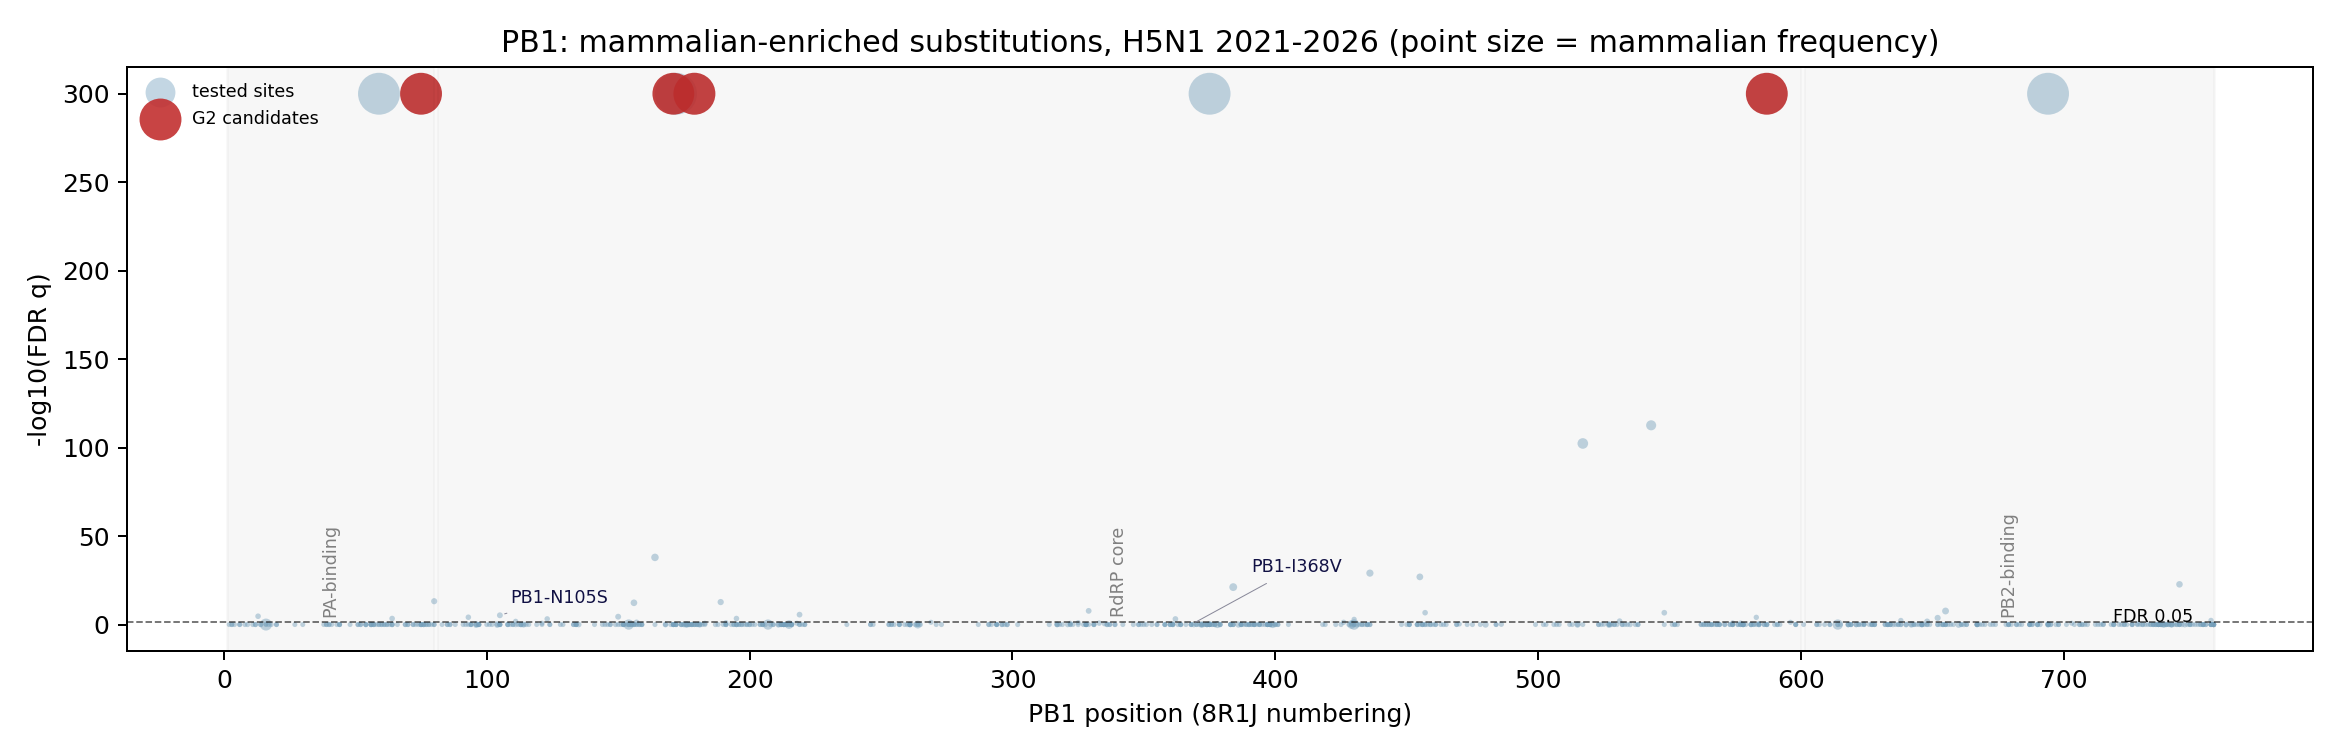
\includegraphics[width=\textwidth]{../results/fig_manhattan_PB1.png}
\caption{PB1 enrichment landscape. Point size = mammalian frequency; red = G2 candidates (all Class L lineage markers).}
\end{figure}
\begin{figure}[!htbp]\centering
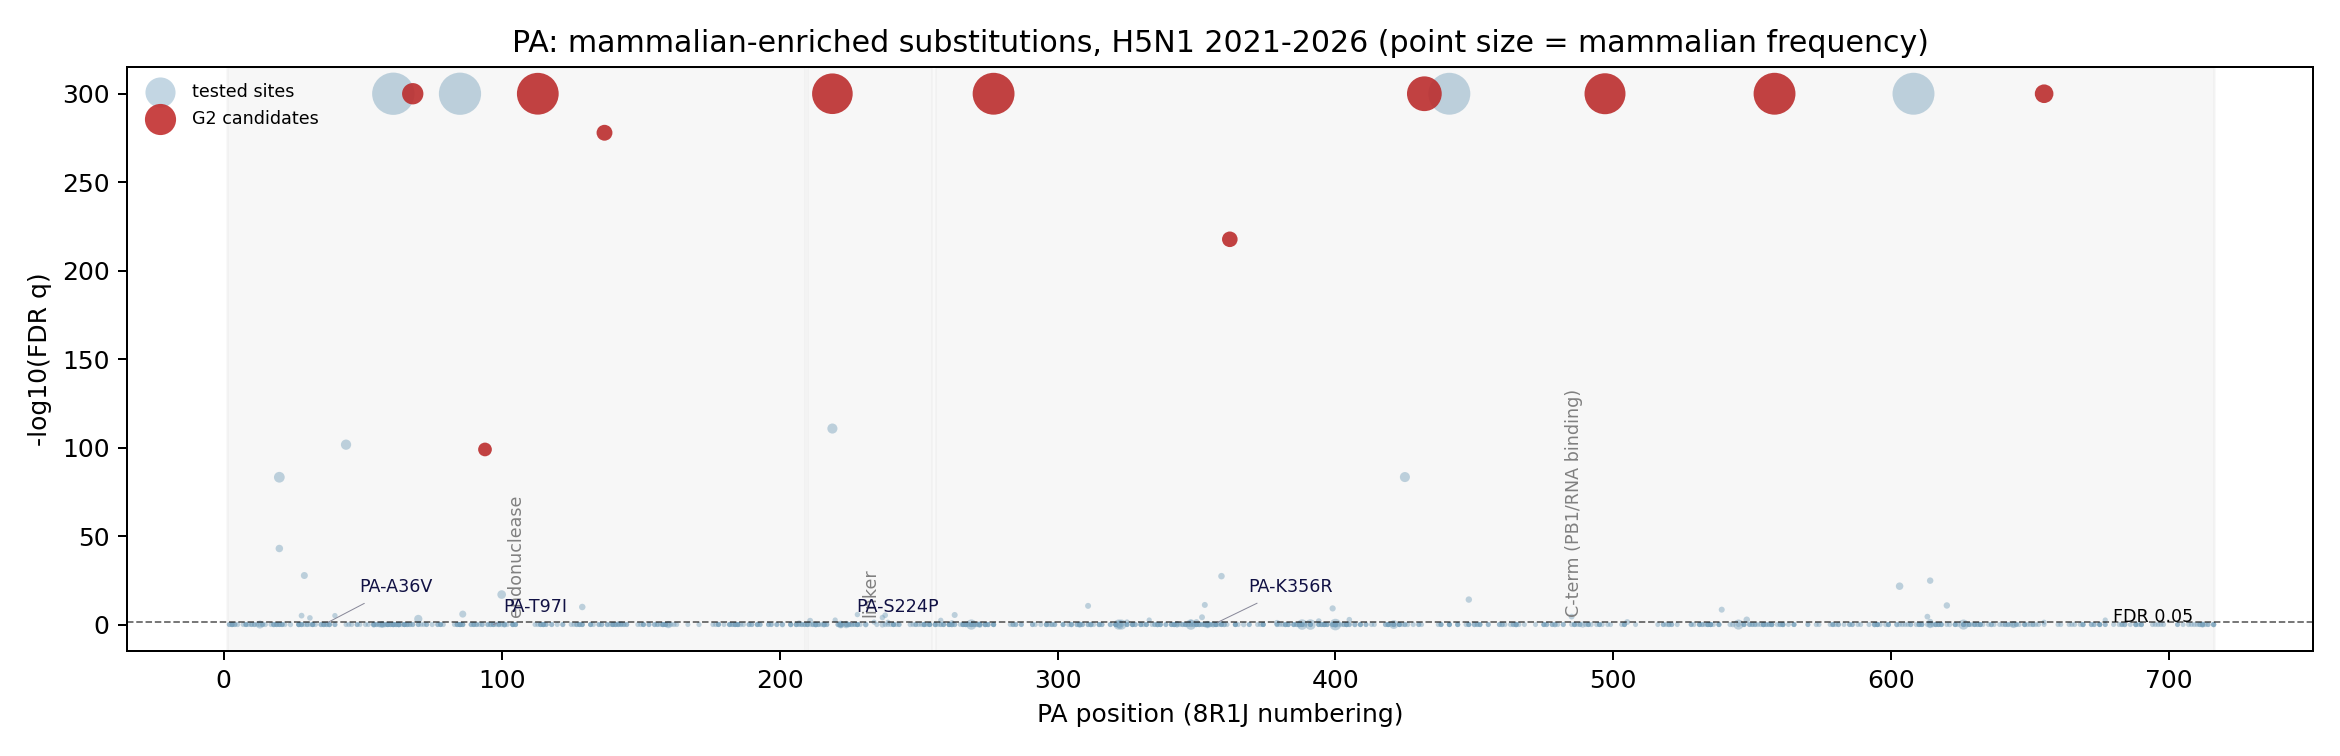
\includegraphics[width=\textwidth]{../results/fig_manhattan_PA.png}
\caption{PA enrichment landscape. Curated marker positions annotated.}
\end{figure}
\begin{figure}[!htbp]\centering
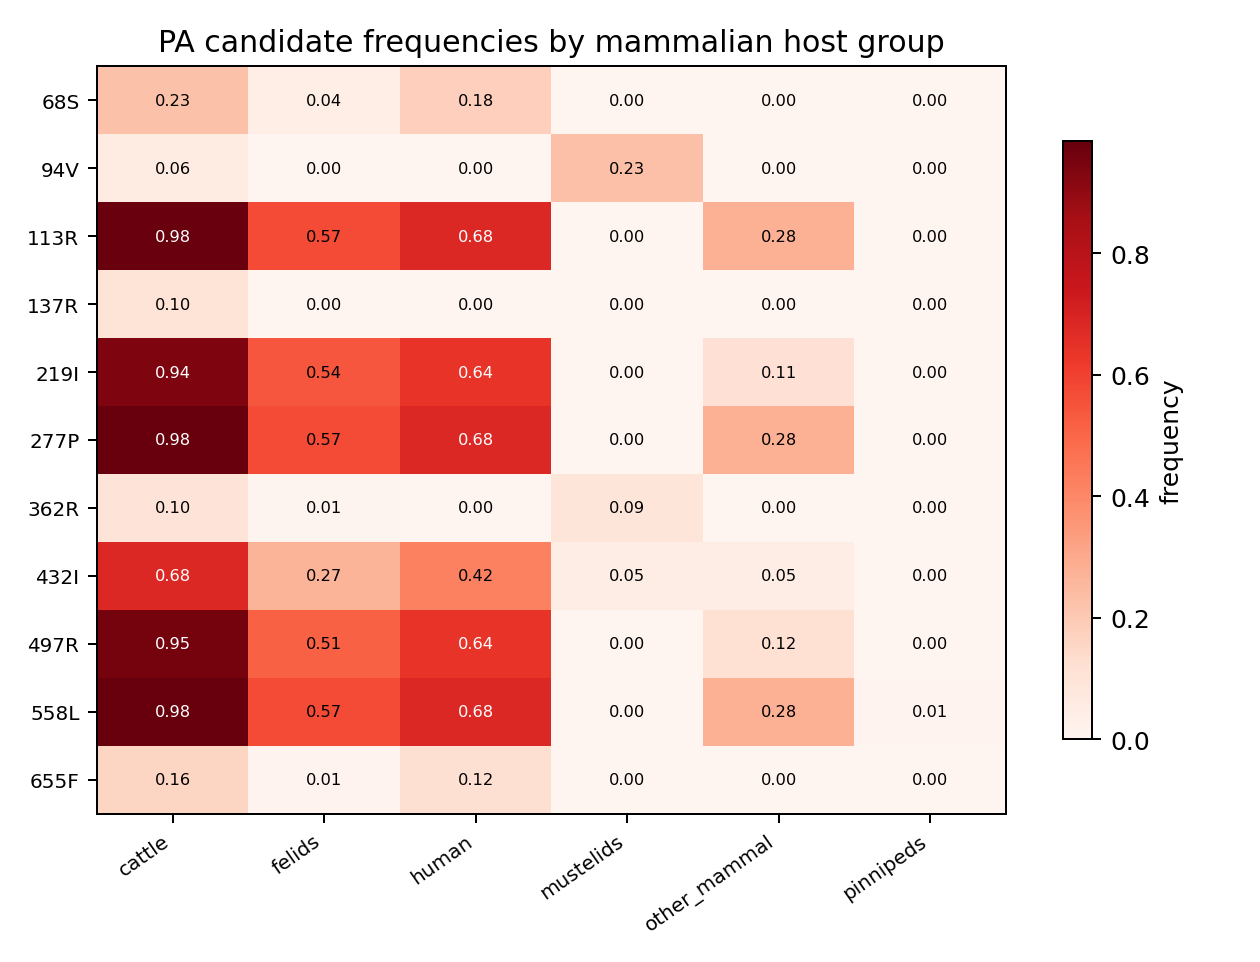
\includegraphics[width=0.8\textwidth]{../results/fig_heatmap_PA.png}
\caption{PA candidate frequencies by mammalian host group. The cattle-dominated cluster with 0\% pinniped carriage (rows 2,3,4,6,7) marks B3.13 genotype markers; polymorphic rows (P68S, V432I, L655F) are outbreak-emergent.}
\label{fig:heat}
\end{figure}
\begin{figure}[h]
\centering
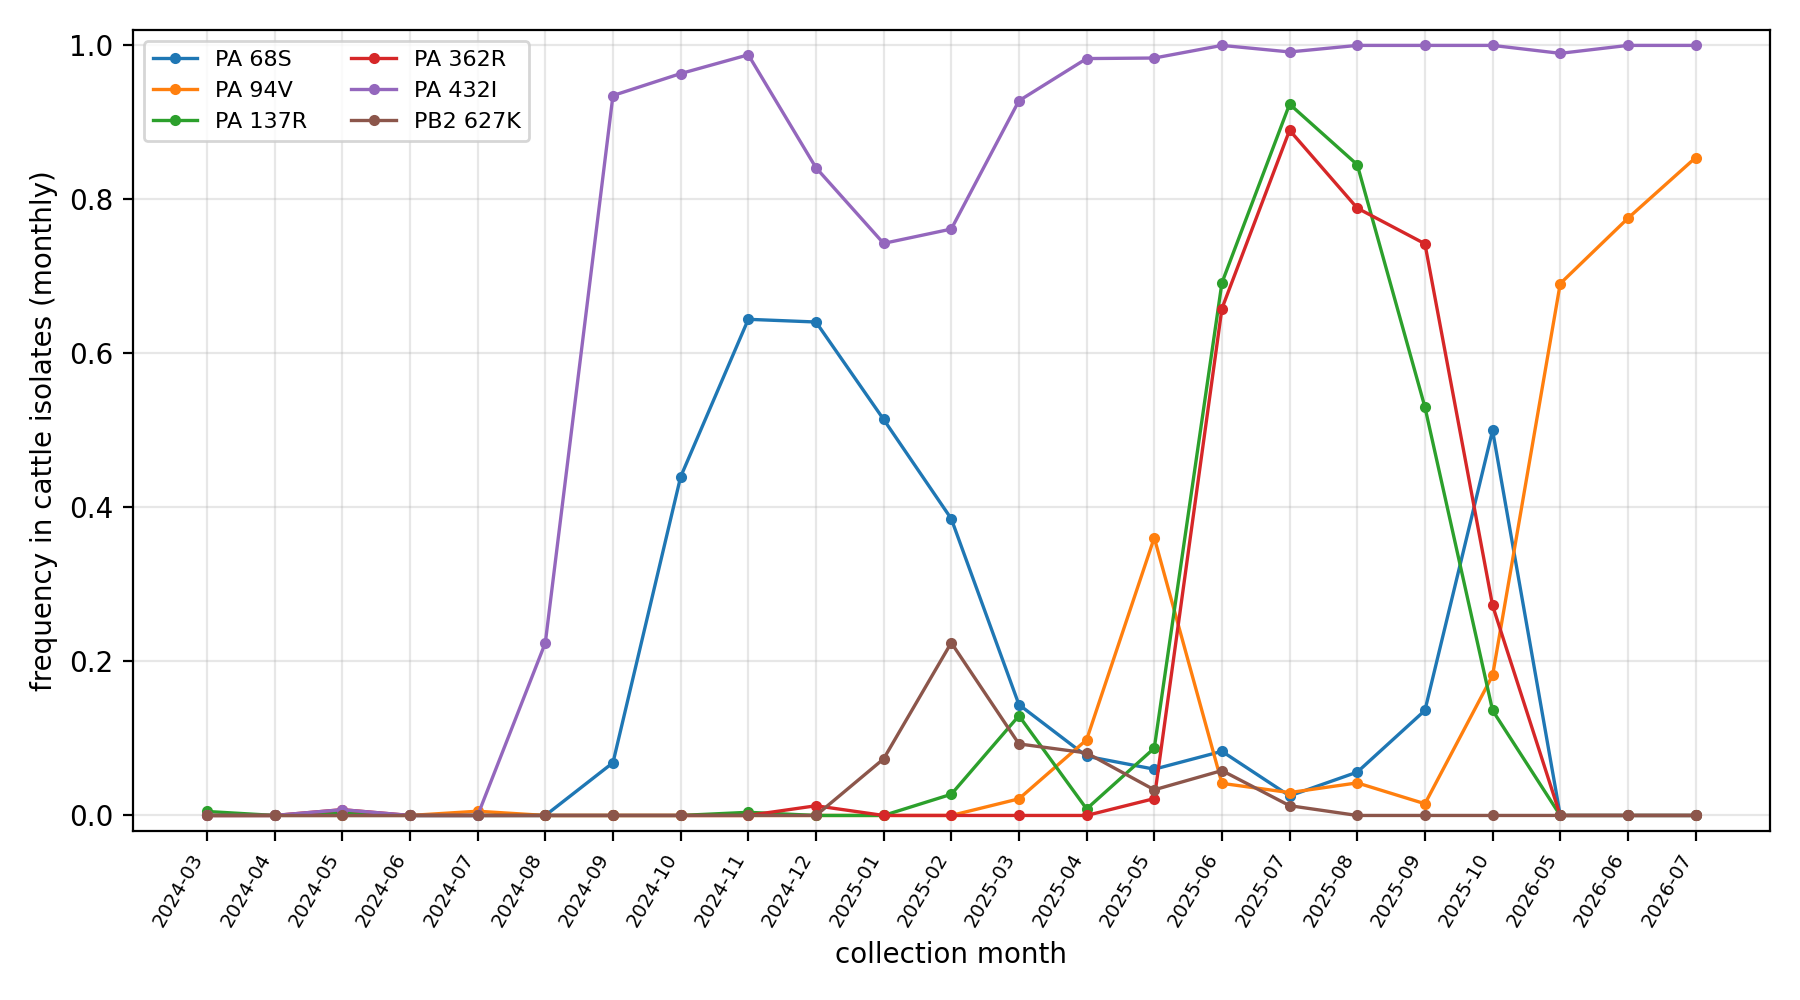
\includegraphics[width=\textwidth]{../results/fig_temporal.png}
\caption{Monthly frequencies of candidate PA alleles and PB2 E627K in bovine H5N1 isolates (months with $\geq$10 sequences). Successive waves of P68S (late 2024), K362R (mid 2025), and I94V (2026) indicate lineage replacement; V432I is fixed since early 2025; E627K did not persist.}
\label{fig:temporal}
\end{figure}
\begin{figure}[!htbp]\centering
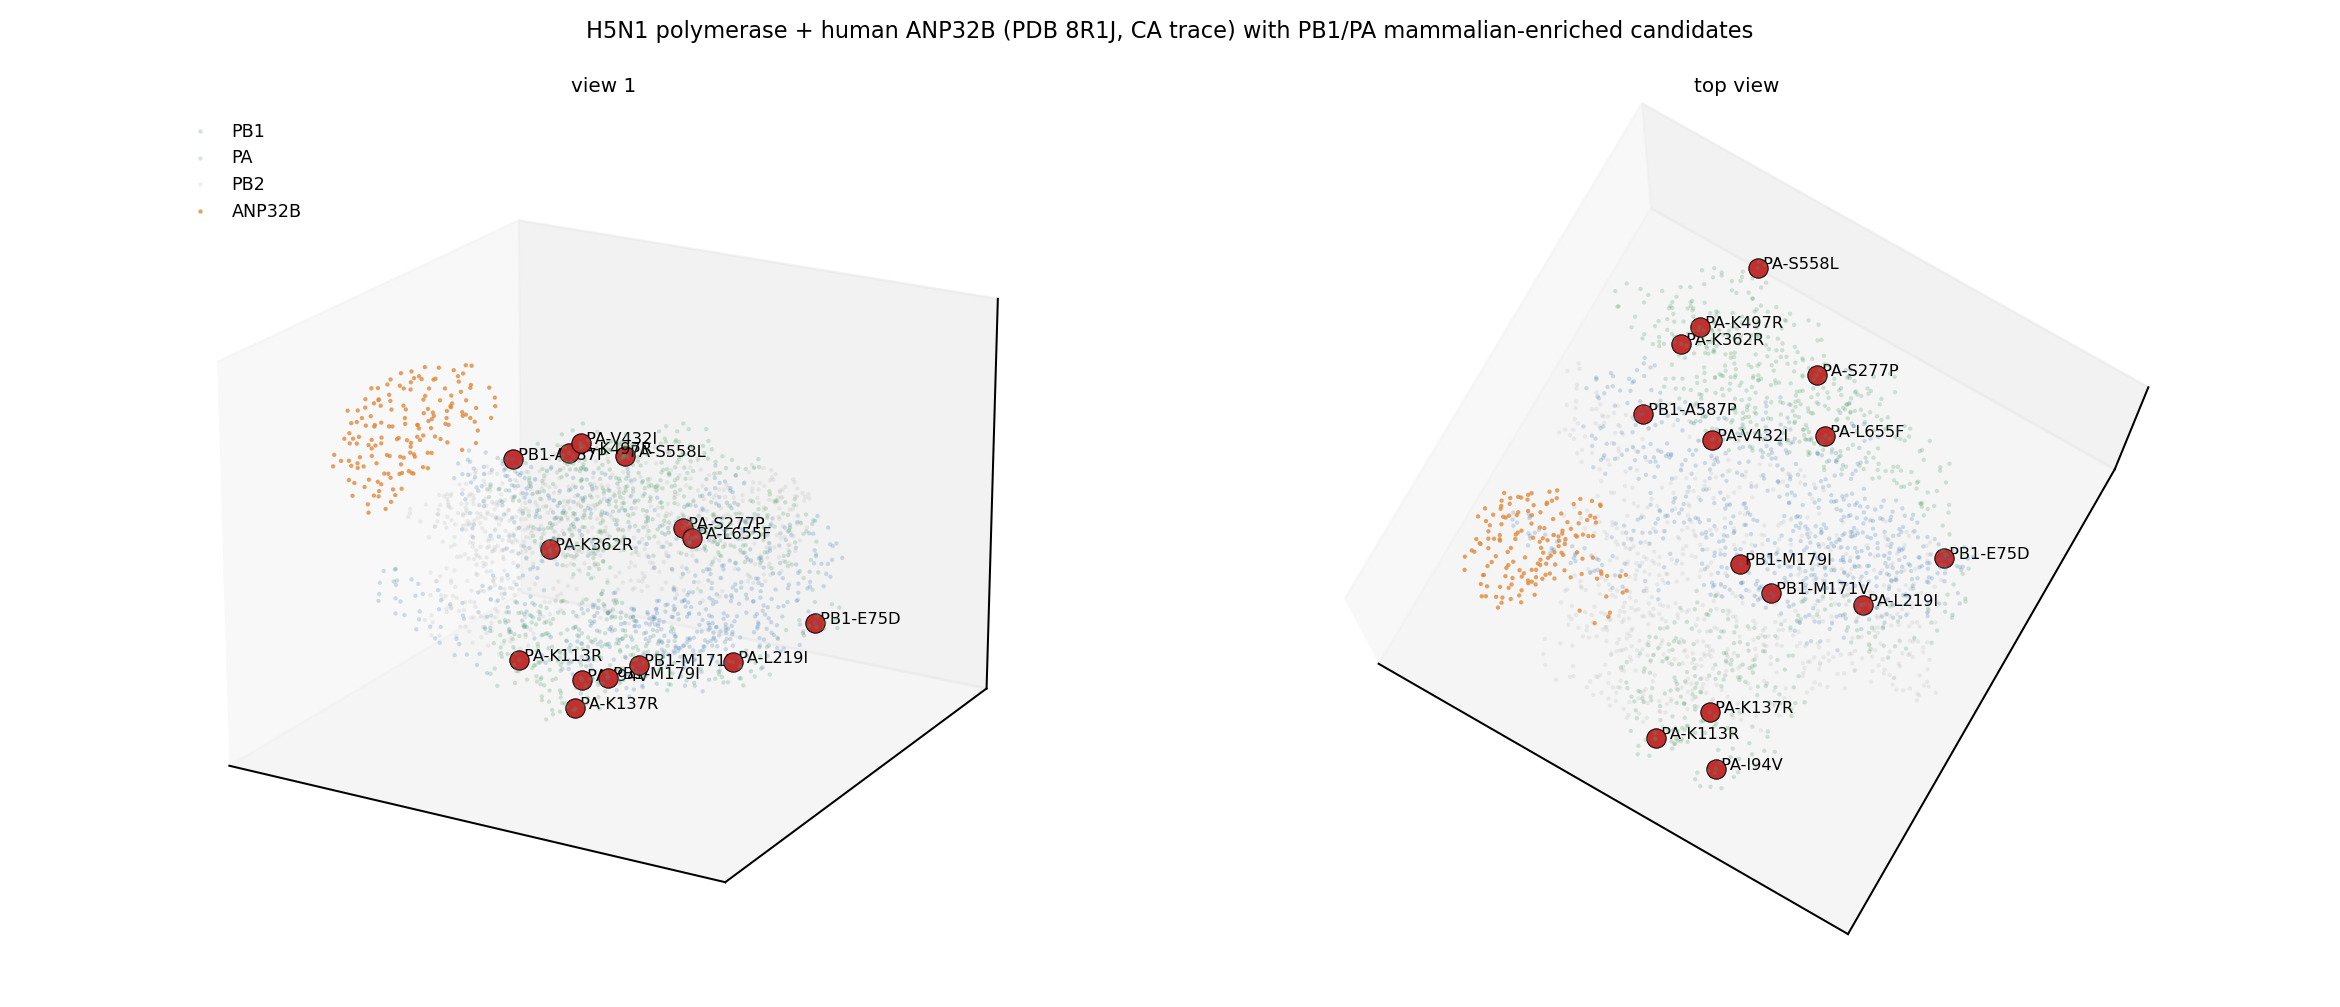
\includegraphics[width=\textwidth]{../results/fig_structure3d.png}
\caption{C$\alpha$ trace of the H5N1 polymerase (PB1 blue, PA green, PB2 grey) with human ANP32B (orange), PDB 8R1J. Red spheres: PB1/PA candidates.}
\end{figure}

\section{Discussion}
Three conclusions emerge. First, \textbf{the historical marker framework misclassifies the current lineage.} Five of eleven literature markers are fixed in avian 2.3.4.4b, one validated marker (T97I) is absent, and one (N66S) is inverted. Risk-assessment panels that count these markers will overstate the adaptation of avian field isolates and under-resolve the changes that actually matter now. Second, \textbf{the dominant signal in mammalian H5N1 genomes today is founder effect, not adaptation.} Every high-frequency ``enrichment'' in PB1 and the PA C-terminus is a fixed marker of the B3.13 cattle genotype, absent from the independently mammal-adapted pinniped lineage. Studies without an independent-lineage control will misread these as adaptation. Third, \textbf{the live adaptation signal is outbreak-emergent and structurally coherent}: PA P68S at the ANP32B interface (8.3\,\AA{}), V432I at the PB2 interface (8.4\,\AA{}), and the cross-lineage convergence of I94V and K362R in cattle and mustelids. These are the priority candidates for experimental polymerase-activity assays in mammalian cells.

\section{Limitations}
(i) Cattle constitute $\approx$85\% of mammalian sequences; non-cattle groups are small (mustelids $n=22$, humans $n\approx50$), so convergence signals rest on modest counts and require phylogenetic confirmation with tree-based methods. (ii) GenBank under-represents GISAID-only submissions; host and date metadata are submitter-supplied. (iii) Genotype assignment here is by host-group proxy, not full phylogenetic typing; B3.13 membership of individual avian sequences was not resolved. (iv) Structural interpretation uses a single complex (8R1J/8R1L); side-chain effects are inferred from C$\alpha$ geometry only. (v) PB1-F2 analyses are complicated by frequent truncations and 71\% median identity to the reference.

\section{Conclusions}
Locked-gate, byte-locked analysis of 71,778 H5N1 records shows that clade 2.3.4.4b is pre-adapted at historical PB1/PA marker positions, that the largest mammalian enrichments are cattle-genotype founder markers, and that the credible current adaptation candidates are outbreak-emergent PA substitutions---above all P68S at the human ANP32B interface and the cross-lineage convergent I94V/K362R. All gates, controls, negative results, code, and checksums are preserved in the repository.

\begin{thebibliography}{9}\small
\bibitem{gabriel2015} Gabriel G et al. Identification of mammalian-adapting mutations in the polymerase complex of an avian H5N1 influenza virus. \emph{Nat Commun} 2015. \url{https://www.nature.com/articles/ncomms8491}
\bibitem{h6n1} PB2-E627K and PA-T97I substitutions enhance polymerase activity and confer a virulent phenotype to an H6N1 avian influenza virus in mice. \emph{Virology} 2014. \url{https://pubmed.ncbi.nlm.nih.gov/25194918/}
\bibitem{conenello} Conenello GM et al. A single mutation in the PB1-F2 of H5N1 (HK/97) and 1918 influenza A viruses contributes to increased virulence. \emph{PLoS Pathog} 2007. \url{https://journals.plos.org/plospathogens/article?id=10.1371/journal.ppat.0030141}
\bibitem{inventory} Molecular signatures of mammalian adaptation of avian influenza viruses (inventory built on Suttie et al., Virus Genes 2019; updated July 2024). \url{https://www.mcmasterforum.org/docs/default-source/product-documents/rapid-responses/molecular-signatures-of-mammalian-adaptation-of-avian-influenza-viruses.pdf}
\bibitem{ph1n1sig} Genomic signatures of influenza A pandemic (H1N1) 2009 virus. \emph{Emerg Infect Dis} 2009. \url{https://wwwnc.cdc.gov/eid/article/15/12/09-0845_article}
\bibitem{mehle} Mehle A, Doudna JA. Adaptive strategies of the influenza virus polymerase for replication in humans. \emph{PNAS} 2009. \url{https://www.pnas.org/doi/10.1073/pnas.0904097106}
\bibitem{structure} Structures of H5N1 influenza polymerase with ANP32B reveal mechanisms of genome replication and host adaptation. \emph{Nat Commun} 2024. \url{https://doi.org/10.1038/s41467-024-48470-3} (PDB 8R1J, 8R1L)
\bibitem{finkelstein} Finkelstein DB et al. Persistent host markers in pandemic and H5N1 influenza viruses. \emph{J Virol} 2007. \url{https://pubmed.ncbi.nlm.nih.gov/17652405/}
\bibitem{spectrum} Decoding non-human mammalian adaptive signatures of 2.3.4.4b H5N1 to assess its human adaptive potential. \emph{Microbiol Spectr} 2025. \url{https://doi.org/10.1128/spectrum.00948-25}
\bibitem{genomicsig} Genomic signatures and host adaptation of H5N1 clade 2.3.4.4b (2025). \url{https://www.sciencedirect.com/science/article/pii/S2666517425000392}
\end{thebibliography}
\end{document}
